\documentclass[11pt,letterpaper]{article}                  % Define document class

%\usepackage{amsfonts} % For \mathbb command
%\usepackage[top=1in, bottom=1.25in, left=1in, right=1in]{geometry}
%\usepackage{amsmath} % for align
%\usepackage{mathtools} % for lVert
%\usepackage{graphicx} % for charts

% Set path
\newcommand{\path}{Preamble}

% Text packages
% Text packages
\usepackage[margin=1in]{geometry}                          % Margin size
\usepackage{enumerate}                                     % Custom enumeration lists
\usepackage{footmisc}                                      % Stable footnotes in headings
\usepackage{natbib}                                        % Bibliography
\usepackage{hyperref}                                      % Hyperreferences
    \hypersetup{
      colorlinks,
      citecolor=black,
      filecolor=black,
      linkcolor=black,
      urlcolor=blue
    }
\usepackage[]{authblk}                                     % Affiliation in maketitle
    \renewcommand\Affilfont{\small}                        % Small font size for affiliation
\usepackage{multicol}                                      % Multiple columns in text
\usepackage[nointegrals]{wasysym}                          % WASY2 symbols for contradiction \lightning
\usepackage{lmodern}                                       % Latin Modern font for correct T1 font encoding (no pixelated output)
\usepackage{algorithm}                                     % Pseudocode packages
\usepackage{algpseudocode}
\setlength\parindent{0pt}                                  % No indentation for the whole document

% Figure/table packages
% Figure and table packages
\usepackage{float}                                         % Figure floats
\usepackage[position=top]{subfig}                          % Subfigures
\usepackage{multirow}                                      % Merged rows in tables
\usepackage{dcolumn}                                       % Custom table delimiters
\usepackage{epstopdf}                                      % EPS files saved as PDF
\usepackage[labelfont=bf, font=normalsize]{caption}        % Bold captions
    \captionsetup{format=hang}

% Math packages
% Math packages
\usepackage{amsmath}                                       % AMS math package
\usepackage{amssymb}                                       % Math symbols
\usepackage{amsthm}                                        % Custom theorem environments
\usepackage{units}                                         % Numerical fractions
\usepackage{centernot}                                     % Logical negation in the middle of characters; e.g. not iff

% Custom theorems
% E.g. \newtheorem{command}[counter]{Display name}
\newtheorem{theorem}{Theorem}[]
\newtheorem{acknowledgement}[theorem]{Acknowledgment}
\newtheorem{axiom}[theorem]{Axiom}
\newtheorem{case}[theorem]{Case}
\newtheorem{claim}[theorem]{Claim}
\newtheorem{conclusion}[theorem]{Conclusion}
\newtheorem{condition}[theorem]{Condition}
\newtheorem{conjecture}[theorem]{Conjecture}
\newtheorem{corollary}[theorem]{Corollary}
\newtheorem{criterion}[theorem]{Criterion}
\newtheorem{exercise}[theorem]{Exercise}
\newtheorem{lemma}[theorem]{Lemma}
\newtheorem{notation}[theorem]{Notation}
\theoremstyle{definition}
\newtheorem*{definition}{Definition}
\newtheorem*{altdef}{Alternative definition}
\newtheorem{problem}[theorem]{Problem}
\newtheorem{assumption}[theorem]{Assumption}
\newtheorem{proposition}[theorem]{Proposition}
\theoremstyle{remark}
\newtheorem{example}[theorem]{Example}
\newtheorem{remark}[theorem]{Remark}
\newtheorem{solution}[theorem]{Solution}
\newtheorem{summary}[theorem]{Summary}

\renewcommand{\qedsymbol}{$\blacksquare$}                  % QED

% Mathematical operators
\DeclareMathOperator{\E}{E}                                % Expected value
\DeclareMathOperator{\var}{var}                            % Variance
\DeclareMathOperator{\cov}{cov}                            % Covariance
\DeclareMathOperator{\corr}{corr}                          % Correlation
\DeclareMathOperator{\avar}{avar}                          % Asymptotic variance
\DeclareMathOperator{\plim}{plim}                          % Probability limit
\DeclareMathOperator{\lag}{lag}                            % Lag operator
\DeclareMathOperator{\rank}{rank}                          % Rank
\DeclareMathOperator{\I}{I}                                % Identity matrix

\providecommand{\abs}[1]{\left\lvert#1\right\rvert}        % Absolute value
\providecommand{\norm}[1]{\left\lVert#1\right\rVert}       % Norm
\providecommand{\ip}[1]{\left\langle#1\right\rangle}       % Inner product
\providecommand{\csp}{\overline{\mathrm{sp}}}              % Closed span
\providecommand{\pto}{\overset{p}{\to}}                    % Convergence in probability
\providecommand{\dto}{\overset{d}{\to}}                    % Convergence in distribution

% Graphics packages
% Graphics packages
\usepackage{tikz}                                          % TikZ drawings
\usepackage{pgfplots}                                      % PGFPlots plots
    \pgfplotsset{                                          % PGFPlots options
        cartesian/.style={                                 % Declaring Cartesian plane style
            % Axis alignment
            axis x line=middle,
            axis y line=middle,
            % Axis labels alignment
            every axis x label/.style={at={(current axis.right of origin)},anchor=north west},
            every axis y label/.style={at={(current axis.above origin)},anchor=north east},
            % Legend alignment
            every axis legend/.append style={legend pos=outer north east}
        },
        % Version declaration for compatibility
        compat=1.11
    }
\usetikzlibrary{calc}
    % Node setup for extensive form games
    \tikzset{
        % Two node styles for game trees: solid and hollow
        solid node/.style={circle,draw,inner sep=1.5,fill=black},
        hollow node/.style={circle,draw,inner sep=1.5},
        % Solution nodes
        solidsol node/.style={blue,circle,draw,inner sep=1.5,fill=blue},
        hollowsol node/.style={blue,circle,draw,inner sep=1.5}
    }

\allowdisplaybreaks % so that aligned equations can be broken across pages

%% Convenient math abbreviations
\newcommand*\diff{\mathop{}\!d} % nicely formatted integral dx
%\newcommand{\E}{\mathrm{E}} % Expectation operator
\newcommand{\Var}{\mathrm{Var}} % Variance operator
\newcommand{\Cov}{\mathrm{Cov}} % Covariance operator
%\newtheorem{problem}{Problem}
%\DeclarePairedDelimiter\norm{\lVert}{\rVert} % For Euclidean norm


% Title
\title{Problem Set 1 \\ \medskip \Large{Econometrics III}}
\author{\Large Jackson Bunting, Attila Gyetvai, Peter Horvath, Leonardo Salim Saker Chaves\footnote{Department of Economics, Duke University}}
\date{\today}

%%%%%%%%%%%%%%%%%%%%%%%%%%%%%%%%%

\begin{document}

\maketitle
%1
\begin{problem}
Verify that the uniform metric defined as $d (f, g) = \sup\limits_{t \in \mathbb{T}} |f(t) - g(t)|, \:  f, g \in l^{\infty}(\mathbb{T})$ is indeed a metric. \\

\textbf{Solution:} Let $f(t), g(t), h(t) \in l^{\infty}(\mathbb{T})$. We will show that the uniform metric satisfies the definition of a metric. That is, 
\begin{enumerate}
	\item  $\sup\limits_{t \in \mathbb{T}} |f(t) - g(t)| = 0$ if and only if $f(t) = g(t)$ since $|\cdot| \geq 0$ and $|a| = 0$ if and only if $a = 0$
	\item  $|f(t) - g(t)| = |g(t) - f(t)|$, therefore $\sup\limits_{t \in \mathbb{T}} |f(t) - g(t)| = \sup\limits_{t \in \mathbb{T}} |g(t) - f(t)|$
	\item $|f(t) - g(t)| = |f(t) - h(t) + h(t) - g(t)| \leq |f(t) - h(t)| +  |h(t) - g(t)|$ by triangle inequality. Therefore, $\sup\limits_{t \in \mathbb{T}} |f(t) - g(t)| \leq  \sup\limits_{t \in \mathbb{T}} |f(t) - h(t)| + \sup\limits_{t \in \mathbb{T}} |h(t) - g(t)|$
\end{enumerate}
\end{problem}

\bigskip
%2
\begin{problem}

\end{problem}

\bigskip
%3
\begin{problem}
Let $\{X_i\}_{i \in \mathbb{N}}$ be a sequence of random variables with mean $\mu$. Suppose that $Cov(X_t,X_s)=0 \forall t\neq s$ and $Var(X_t) \leq Kt^{1/2}$ for some constant $K>0$. Show that $\bar{X_t} \overset{\mathbb{P}}{\rightarrow} \mu$.\\

\textbf{Solution:} Consider any $\epsilon>0$. Using Markov inequality we get
\begin{align*}
P(|\bar{X_t} - \mu| > \epsilon) &\leq \frac{\mathbb{E}( |\bar{X_t} - \mu|^2)}{\epsilon^2} = \frac{V(\bar{X_t})}{\epsilon^2} \\
&\leq \frac{\sum_{t=1}^T V(X_t)}{T^2 \epsilon^2} = \frac{K \sum_{t=1}^T t^{1/2}}{T^2 \epsilon^2} \\
&\leq \frac{K T^{3/2}}{T^2 \epsilon^2} \overset{t \to \infty}{\longrightarrow} 0
\end{align*}

Then $\bar{X_t} - \mu \overset{\mathbb{P}}{\rightarrow} 0$ which is equivalent to what we wanted to show.
\end{problem}

\bigskip
%4
\begin{problem}

\end{problem}

\bigskip
%5
\begin{problem}
Suppose that $\sup_{t \in \mathcal{T}} \mathbb{E}(|X_t|^{1+\delta}) < \infty$ for some $\delta >0$. Then $\{X_t : t \in \mathcal{T}\}$ is uniformly integrable. (Hint: Markov's inequality) \\

\textbf{Solution:} Notice that $\frac{|X_t|}{M} \geq I[|X_t|>M] \implies \frac{|X_t|^{\delta}}{M^{\delta}} \geq I[|X_t|>M]$. 

Using that $|X_t|\geq 0$,
\begin{align*}
&\frac{|X_t|^{1+\delta}}{M^{\delta}}\geq |X_t| I[|X_t|>M] \forall \ t \in \mathcal{T}\\
&\implies \sup_{t \in \mathcal{T}} \mathbb{E}(|X_t|^{1+\delta}) (1/M^{\delta}) \geq \sup_{t \in \mathcal{T}} \mathbb{E}(|X_t|I[|X_t|>M]) \forall \ M \in \mathbb{N} \\
&\implies \lim_{M \to \infty} \sup_{t \in \mathcal{T}} \mathbb{E}(|X_t|^{1+\delta}) (1/M^{\delta}) = 0 \geq \lim_{M \to \infty} \sup_{t \in \mathcal{T}} \mathbb{E}(|X_t|I[|X_t|>M]) \geq 0
\end{align*}
The inequalities above give that $X_t$ is uniformly integrable.
\end{problem}

\bigskip

%6
\begin{problem}
Suppose that $|X_t| \leq Y$ for some integrable random variable $Y$ and all $t \in \mathbb{T}$.
Then $\{ X_t: t \in \mathbb{T} \}$ is uniformly integrable. \\

\textbf{Solution:} 

\begin{align*}
	|X_t| &\leq Y \\
	\implies |X_t| 1_{\{ |X_t| \geq M \}} &\leq Y 1_{\{ Y \geq M \}} \\
	\implies \mathbb{E} \left[ |X_t| 1_{\{ |X_t| \geq M \}} \right] &\leq \mathbb{E} \left[ Y 1_{\{ Y \geq M \}} \right] \\
	\implies \sup_{t \in \mathbb{T}} \mathbb{E} \left[ |X_t| 1_{\{ |X_t| \geq M \}} \right] &\leq \sup_{t \in \mathbb{T}} \mathbb{E} \left[ Y 1_{\{ Y \geq M \}} \right] = \mathbb{E} \left[ Y 1_{\{ Y \geq M \}} \right] \\
	\implies \lim_{M \to \infty} \sup_{t \in \mathbb{T}} \mathbb{E} \left[ |X_t| 1_{\{ |X_t| \geq M \}} \right] &\leq \underbrace{\lim_{M \to \infty} \mathbb{E} \left[ Y 1_{\{ Y \geq M \}} \right]}_{= 0 \text{ as $Y$ is integrable}} \\
	\implies \lim_{M \to \infty} \sup_{t \in \mathbb{T}} \mathbb{E} \left[ |X_t| 1_{\{ |X_t| \geq M \}} \right] &= 0
	\intertext{The second line follows from the fact that the indicator function is stricly increasing.
	The third line follows from the fact that expectation is strictly increasing.}
\end{align*}
\end{problem}

\bigskip

%7
\begin{problem} (Characteristic Function) Let $X_n$ and $X$ be $\mathbb{R}^d$-valued random variables. Suppose that $X_n \Rightarrow X$. Show that for any $\theta \in \mathbb{R}^d$, we have the following:
	(a) $\mathbb{E}\left[\cos(\theta' X_n)\right] \rightarrow \mathbb{E}[\cos(\theta' X)]$
	(b) $\mathbb{E}[\sin(\theta' X_n)] \rightarrow \mathbb{E}[\sin(\theta' X)]$;
	(c) the characteristic function of $X_n$ converges to the characteristic function of $X$. \\
	
\textbf{Solution:} 

(a) 	$f(x) = \cos(x)$ is a continuous bounded function on $\mathbb{R}$. Invoking the definition of weak convergence, we get that $\mathbb{E}\left[\cos(\theta' X_n)\right] \rightarrow \mathbb{E}[\cos(\theta' X)]$ since $X_n \Rightarrow X$. \\
	
(b) 	$f(x) = \sin(x)$ is a continuous bounded function on $\mathbb{R}$. Invoking the definition of weak convergence, we get that $\mathbb{E}[\sin(\theta' X_n)] \rightarrow \mathbb{E}[\sin(\theta' X)]$ since $X_n \Rightarrow X$. \\

(c) The characteristic function of $Y$ random variable is $\phi_{Y}(t) = \mathbb{E}\left[\exp(itY)\right] = \mathbb{E}(\cos(tY) + i \sin(tY))$. From (a) and (b), it follows that  $\phi_{X_n}(t) =  \mathbb{E}(\cos(tX_n) + i \sin(tX_n)) = \mathbb{E}(\cos(tX_n)) + i \mathbb{E}(\sin(tX_n)) \rightarrow \mathbb{E}(\cos(tX)) + i \mathbb{E}(\sin(tX)) = \phi_{X}(t).$

\end{problem}

\bigskip

%8
\begin{problem}(Laplace Transform) Let $X_n$ and $X$ be $\mathbb{R}_{+}$-valued random variables. Suppose that $X_n \Rightarrow X$. Show that for any $\theta \geq 0$, we have $\mathbb{E}(\exp(-\theta X_n)) \rightarrow \mathbb{E}(\exp(-\theta X))$ \\
	
\textbf{Solution:} 

$f(x) = \exp(-\theta x)$ is a bounded continuous function on $\mathbb{R}_{+}$ if $\theta \geq 0$. Therefore, we can use the definition of weak convergence to get $\mathbb{E}(\exp(-\theta X_n)) \rightarrow \mathbb{E}(\exp(-\theta X))$ as   $X_n \Rightarrow X$.

\end{problem}

\bigskip

%9
\begin{problem} Let $X_n$ and $X$ be real-valued random variables with $X_n \xrightarrow{a.s.} X.$ Let $r \in \mathbb{R}$ with $\mathbb{P}(X = r) = 0$. Show that 
	(a) $1_{X_n \leq r} \xrightarrow{a.s.} 1_{X \leq r}$;
	(b) $\mathbb{P}(X_n \leq r) \rightarrow \mathbb{P}(X \leq r)$. (Hint: bounded convergence theorem).
	Show (b) but assume $X_n \Rightarrow X$ instead of $X_n \xrightarrow{a.s.} X.$ (Hint: Almost sure representation) \\
	
\textbf{Solution:}	

	(a) $f(x) = 1_{x \leq r}$ is only discontinuous at r, otherwise it is continuous on the real line. However, $\mathbb{P}(X = r) = 0$, therefore we can apply continuous mapping theorem. That is, if $X_n \xrightarrow{a.s.} X$, then $f(X_n) \xrightarrow{a.s.} f(X)$ for $f(x) = 1_{x \leq r}$. \\
	
	(b) From (a), we know that $1_{X_n \leq r} \xrightarrow{a.s.} 1_{X \leq r}$ and $|1_{X_n \leq r}| \leq Y = 2$ for every $n \in \mathbb{N}$ (i.e. $Y$ is some integrable variable). So we can invoke dominated convergence theorem to get that $\mathbb{P}(X_n \leq r) = \mathbb{E}\left[1_{X_n \leq r}\right] \xrightarrow{a.s.} \mathbb{E}\left[1_{X \leq r}\right] = \mathbb{P}(X \leq r)$. \\ 
	
	(c) Since $X_n \Rightarrow X$, by almost sure representation, $\exists \left( (\tilde{X}_n)_{n \in \mathbb{N}} \text{ and } \tilde{X} \right)$, such that $X_n \sim \tilde{X}_n, X \sim \tilde{X}$ and $\tilde{X}_n \xrightarrow{a.s.} \tilde{X}.$ From (a) and (b), we know that for $\tilde{X}_n$ and $\tilde{X}$, that $\mathbb{P}(\tilde{X}_n \leq r) \rightarrow \mathbb{P}(\tilde{X} \leq r)$. Since $X_n \sim \tilde{X}_n, X \sim \tilde{X}$, we have that $\mathbb{P}(\tilde{X}_n \leq r) = \mathbb{P}(X_n \leq r)$ and $\mathbb{P}(\tilde{X} \leq r) = \mathbb{P}(X \leq r)$.
\end{problem}

\bigskip
%10
\begin{problem}
Let $a_n = o(1)$.
Interpret and prove that $O_p(a_n) = o_p(1)$. \\

\textbf{Solution:} If I divide $X_n$ by $a_n = o(1)$, it has to be the case that $X_n  = o_p(1)$.
The proof is the following:
\begin{align*}
  X_n &= O_p (a_n) \iff \frac{X_n}{a_n} = O_p(1); \\
  X_n &= \frac{X_n}{a_n} \, a_n = O_p(1) \, o(1) \implies O_p(1) o_p(1) = o_p(1)
\end{align*}
The first line is just the definition of $O_p(a_n)$.
The second line comes from the fact that pointwise convergence implies convergence in probability, and the $o_p$--$O_p$ identities in the notes.
\end{problem}

\bigskip
%11
\begin{problem}
Interpret and prove that $e^{o_p(1)} -1 = o_p(1)$ and $(O_p(1))^{\sqrt{2}} = O_p(1)$. \\

\textbf{Solution:} If you pick a r.v. $X = o_p(1)$, then a continuous transformation will also be $o_p(1)$. The proof is a straightforward consequence of CMT.

For the second claim, the interpretation is that you preserve $O_p(1)$ property when you take a continuous function of this r.v.. To prove, let $X_n = O_p(1)$. By definition, $\exists M>0 ; \sup_{n \in \mathbb{N}} P(|X_n|>M)<\epsilon)$. Notice that $\{\omega \in \Omega : |X_n(\omega)|>M\} = \{\omega \in \Omega : |X_n(\omega)|^{\sqrt{2}}>M^{\sqrt{2}}\}$ because it is a monotonic transformation. Thus, $\exists \eta = M^{\sqrt{2}}>0 ; \sup_{n \in \mathbb{N}} P(|X_n^{\sqrt{2}}|>\eta)<\epsilon)$.
\end{problem}

\bigskip
%12
\begin{problem}
Let $f(x) = \exp (x^2)$.
Let $(X_i)_{1 \leq i \leq n}$ be iid $N(\mu,1)$ variables.
Simulate such a sequence with $n = 100$ and $\mu = 0.3$.
Compute $f (\bar{X}_n)$ where $\bar{X}_n = \frac{1}{n} \sum_{i=1}^n X_i$.
Repeat this for 2000 times. Plot the distribution of $f (\bar{X})$ in the simulation.
What is the asymptotic distribution of $f (\bar{X})$?
Is the asymptotic distribution a good approximation to the empirical distribution?
Repeat for $\mu =$ 0, 0.1, 0.2, 0.3, 0.4, 0.5.
Discuss the results. \\

\textbf{Solution:}
We calculate the asymptotic distribution of $f(\bar{X}_n)$ using CLT and the delta method.
Since $X_i \sim N(\mu, 1)$, it follows from the CLT that $\sqrt{n} (\bar{X}_n - \mu) \Rightarrow N (0, 1)$.
By the delta method, $\sqrt{n} (\exp(\bar{X}_n^2) - \exp(\mu^2)) \Rightarrow N (0, (2 \mu \exp(\mu^2))^2)$.
When $\mu = 0.3$, $\sqrt{n} (\exp(\bar{X}_n^2) - \exp(0.3^2)) \Rightarrow N (0, 0.43)$.

However, note that when $\mu = 0$, the asymptotic distribution becomes degenerate in which case we use a version of the delta method that relies on a second-order Taylor expansion:
$\sqrt{n} (\exp(\bar{X}_n^2) - \exp(\mu^2)) \Rightarrow \frac{1}{2} \cdot 2 \exp(\mu^2) (2\mu^2 + 1) \cdot \chi^2(1)$.
Hence in the case of $\mu = 0$, $\sqrt{n} (\exp(\bar{X}_n^2)) \Rightarrow \chi^2(1)$.

We plot the simulated distributions below.
As the above analysis suggests, the empirical distribution with $\mu = 0$ resembles the $\chi^2$-distribution.
As $\mu$ increases, the empirical distributions look more and more normal.

\begin{figure}[H]
  \centering
  \caption{Simulated empirical distributions}
  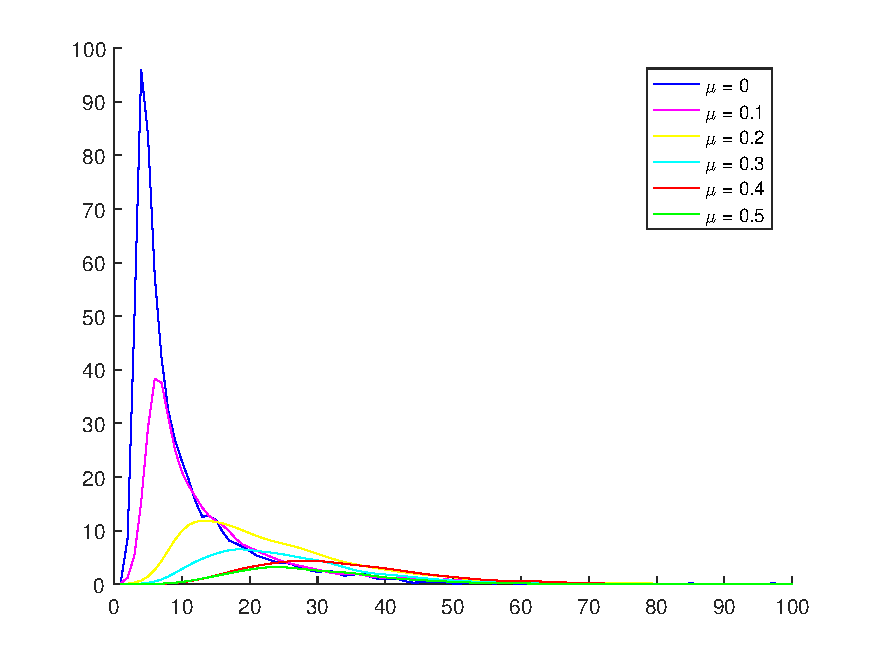
\includegraphics[scale=0.6]{prob12.pdf}
\end{figure}
\end{problem}

\bigskip

%13
\begin{problem}
Let $(X_i)_{i \in \mathbb{N}}$ be a sequence of iid random variables with mean $\mu$ and variance $\sigma^2$. Suppose that for some $\delta>0$, $\mathbb{E}\left[|X_i|^{2+\delta}\right]<\infty$. Use Lindeberg's CLT to show that $n^{1/2}(\frac{1}{n}\sum_{i=1}^{n} X_i - \mu) \implies N(0,\sigma^2)$.

\textbf{Solution:}
Initially consider $X_{n,i} = \frac{X_i - \mu}{\sqrt{n}}$. Now, we need to verify the assumptions of Lindeberg's CLT.
\begin{enumerate}
\item $\{X_{n,i}\}$ independent, real-valued, and zero mean. \\
Since we are applying a continuous function to rv's which are iid by assumption, independence will be preserved. Moreover, considering $X_i:\Omega \mapsto \mathbb{R}$, we will have $X_{n,i}$ real-valued. And notice that $\mathbb{E}[X_{n,i}] = \mathbb{E}[(X_i - \mu)/\sqrt{n}] = 0$.\\ 
\item $\sum_{i=1}^n V(X_{n,i} = \frac{\sum_{i=1}^n \sigma^2}{n} = \sigma^2$
\item $\lim_{n \to \infty} \sum_{i=1}^n \mathbb{E}[X_{n,i}^2 I[|X_{n,i}|>\epsilon]] =0$\\
Using an argument similar to Q5, we have $\frac{|X_{n,i}|^{2+\delta}}{\epsilon^{\delta}} \geq I[|X_{n,i}|>\epsilon]$. Therefore,
\begin{center}
$\frac{\mathbb{E}(|X_i - \mu|^{2+\delta}}{\epsilon^{\delta} n^{1+\delta/2}}) \geq \mathbb{E}(|X_{n,i}|^2 I[|X_{n,i}>\epsilon]) \forall \ i \in \mathbb{N}$
\end{center}
Using iid assumption and $\mathbb{E}\left[|X_i|^{2+\delta}\right]<\infty$ we have:
\begin{align*}
&\frac{\mathbb{E}(|X_i-\mu|^{2+\delta})}{\epsilon^{\delta}n^{\delta/2}}\geq \sum_{i=1}^n \mathbb{E}(|X_{n,i}|^2 I[|X_{n,i}>\epsilon])\\
&\implies \lim_{n \to \infty} \frac{\mathbb{E}(|X_i-\mu|^{2+\delta})}{\epsilon^{\delta}n^{\delta/2}} =0 \geq \lim_{n \to \infty} \sum_{i=1}^n \mathbb{E}(|X_{n,i}|^2 I[|X_{n,i}>\epsilon]) \geq 0
\end{align*}
\end{enumerate}
Finally, we can apply Lindeberg's CLT to get $n^{1/2}(\frac{1}{n}\sum_{i=1}^{n} X_i - \mu) = \sum_{i=1}^n X_{n,i} \implies N(0,\sigma^2)$.
\end{problem}


\end{document}
